\section{Introduction}
%In this chapter, we present our approach to providing a programmable and dynamic framework that can support data-driven applications by extending software-defined environment concepts to drive the process of dynamically composing infrastructure services from multiple providers. The resulting distributed software-defined environment (dSDE) autonomously evolves over the application life cycle while meeting objectives and constraints set by users, applications, and/or resource providers. In Section 3.1.1, we first discuss the requirements for a dSDE followed by a summary of our methodology in Section 3.1.2. We then present the architecture and implementation of the three layers necessary to realize a dSDE in Sections 3.2-3.4. In Section 3.5, we then demonstrate how the three layers work together to provide a dSDE using a rule-engine–based and a constraint-programming–based approaches. Finally, we provide a summary of the chapter in Section 3.6.

\section{Framework}

The R-Pulsar framework has been built using the semantics defined in the previous section. The ambition of R-Pulsar is to implement a software stack that extends cloud capabilities to edge devices, allowing to collect and analyze data closer to the source of information and react autonomously to local events.

R-Pulsar uses a distributed architecture by the means of an overlay network, where each node in the overlay network is called a Rendezvous Point (RP). RPs can be a gateway located at the edge of the network or a server located in the cloud. R-Pulsar targets applications that span the cloud and the edge of the network.

R-Pulsar consists of five layers: (1) the location-aware self-organizing overlay, (2) the content-based routing layer, (3) the serverless messaging layer, (4) the memory-mapped data-processing layer, and (5) the programming abstraction layer.

%Figure \ref{fig:infrastructure} shows underlying areas of research and how they are connected.
%\begin{figure}[!htb]
%  \centering
%  \includegraphics[width=.75\columnwidth]{./fig/overall-architecture.pdf}
%  \caption{An overall layered architecture of edge-based data-intensive IoT system to achieve computing in the continuum.}\label{fig:infrastructure}
%\end{figure}

\subsection{Location-aware Overlay Network Layer}

IoT data comes with temporal and spatial information, which is directly associated with their business value in a given context. Hence, IoT applications must process data in a timely fashion and from proper locations. R-Pulsar presents a location-aware overlay network in conjunction with point quadtrees to logically connect groups of RPs. The RPs are grouped based on the geographical location to guarantee that data gets processed with minimal latencies.

During the initialization of the overlay network, the RP attempts to discover an already existing RP in the system and construct its routing table. The joining RP sends a discovery message to the group. If the message remains unanswered after a duration (in the order of seconds), the RP assumes that it is the first in the system at it becomes the master RP, creating a single overlay network (Peer-to-Peer network).  If an RP responds to the message, they communicate with the master RP, and they are added to the P2P network. Once the initial P2P network has a sufficient number of RPs to guarantee that in case of multiple failures the P2P network will not disappear, the first P2P network will be subdivided into four additional P2P rings, plus an extra ring that will allow all the master RPs of each ring to communicate. To keep track of all the P2P networks, the quadtree data structure is used. In the case of a master RPs failure, a master RP election is performed using the Hirschberg and Sinclair algorithm~\cite{Hirschberg}. 

%The location-aware overlay network layer provides an abstraction to the layers above, consisting of a single operation: \textbf{lookup}(identifier, AR message). Given the location specified in the AR message, the quadtree is used for searching which group of RPs is the closest to the given location. Then the identifier is used to route it in the overlay network. 

\subsection{Content-based Routing Layer}\label{sec:frameworkc}

This layer builds on top of the location-aware overlay to route messages. As mentioned above, the lookup operator provided by the location-aware overlay requires an exact identifier, the AR message and the location to be routed. The content-based routing layer maps AR profiles onto single identifiers or clusters of identifiers to enable informaton discovery using partial knowledge, as described in \cite{SCHMIDT2008962}.

The Hilbert Space Filling Curve (SFC)~\cite{SFC} is used to map the n-dimensional space of the AR profile to the one-dimensional space ID of the location-aware overlay network. Applying the Hilbert mapping to an AR profile consisting of exact keywords only can be mapped to a single point on the SFC. Furthermore, any AR profile containing wildcard or range keywords can be mapped to regions of points in the SFC.

\textbf{Routing using simple keyword tuples:} The routing process consists of two steps. At the first step, a profile containing only exact keywords is 
encoded into a set of ID's, each id represents an exact keyword, then the set of ID's are passed to the SFC to obtain a single ID. This ID is then  used to find the responsible RP in the P2P network. Figure~\ref{fig:profiles}a illustrates this process. \vspace{1ex} 

\textbf{Routing using complex keyword tuples:} Similarly to the first step, a profile containing wildcards, ranges, or both is encoded and a set of ID's for each keyword are obtained and passed to the SFC. The SFC outputs a collection of IDs, using those IDs, the overlay network lookup mechanism routes the message to all responsible RP nodes in the overlay. Figure~\ref{fig:profiles}b illustrates this process.

%The content-based routing layer of the R-Pulsar stack provides an abstraction to the layer above consisting of a single operation, \textbf{deliver}(AR message), where the AR message contains the profile that is used to route the message. The routing process can be classified as simple or complex based on the AR profile. \vspace{1ex}

\subsection{Serverless Messaging Layer}\label{sec:serverless}

Serverless computing is a cloud computing model that aims to abstract server management and low-level infrastructure decisions away from developers. Allowing to deploy and execute pieces of code in response to events without the need to specify IP addresses.

The serverless messaging layer implements the AR interaction model described in section~\ref{sec:semantics} and it consists of two components: the matching engine and the profile manager. The matching engine component is essentially responsible for matching profiles. If the result of the match is positive, then the action field of the incoming message is executed first, followed by the evaluation of the action field in the matched profiles. The profile manager manages locally stored profiles and monitors message credentials and contexts to ensure that related constraints are satisfied.

%The serverless messaging layer offers a single operation to developers, \textbf{post}(AR message), where the AR message contains the profile that is used to route the message. The AR message then is passed to the content-based routing layer and routed to the desired destination.

\subsection{Memory-mapped Streaming Analytics Pipeline}
The data pipeline is responsible for consolidating data from multiple sources, processing the data, and making them available to be used. State-of-the-art data pipelines are known to be data-intensive tasks, resulting in the inability to performing real-time data analytics when deployed on constrained devices. The memory-mapped streaming analytics pipeline layer is motivated to overcome that issue.

The streaming analytics pipeline comprises the following layers: 

\begin{enumerate}

\item The data collection layer gathers data from multiple sources and brings them to the pipeline.
\item The stream processing layer processes the data and performs computations on the collected data.   
\item The data storage and query layer reads and writes data to the main memory and disk.

\end{enumerate}

\vspace{1ex}
\subsubsection{Data Collection Layer}
\hfill\\
Multiple data collection services are available, such as Apache Kafka~\cite{kafka}, Google Pub/Sub~\cite{google}, Amazon Firehose~\cite{amazon}, and Mosquitto~\cite{mosquitto}. Although some are designed to be deployed on edge devices, these services offer limited performance when deployed in constrained devices due to the limited read and write disk speeds.%low disk I/O performance.

We designed and implemented a custom data collection layer designed specifically for constrained devices using a memory-mapped queue. A memory mapped file is a segment of virtual memory that has been assigned a direct correlation with some portion of a file. This file is physically present on disk, which allows the operating system to ensure data access operations with better performance than standard file access. The core principle of the R-Pulsar queue system emerges from the observation that random memory read is about 3.5x faster than sequential disk read, as measured in Table~\ref{tb:table}. 

The trade-off of using a memory mapped data collection system is that operating systems decides when to copy data from the main memory to disk. %Our approach is based on the assumption that the MQTT protocol assumes that the client and the server are generally available~\cite{IBM-MQTT}. 

\begin{table}[h!]
\scalebox{1.2}{
\begin{tabular}{|l|c|c|}
\hline
\multicolumn{1}{|c|}{\textbf{Operation}} & \textbf{Disk} & \textbf{RAM Memory} \\ \hline
Sequential read                          & 18.89 MB/s             & 631.34 MB/s \\ \hline
Sequential write                         & 7.12 MB/s              & 573.65 MB/s \\ \hline
Random read                              & 0.78 MB/s              & 65.96 MB/s              \\ \hline
Random write                             & 0.15 MB/s              & 65.88 MB/s              \\ \hline
\end{tabular}}
\centering

\caption{Measurements of Disk I/O vs RAM memory performance on a Raspberry Pi.} \label{tb:table}
\vspace{-2ex}
\end{table}

\vspace{1.5ex}
\subsubsection{Data Processing Layer}
\hfill\\
R-Pulsar can be used on top of any data processing engine, allowing the end user to choose his or her favorite data-processing engine. The current release of R-Pulsar was validated using Apache Edgent. 

\vspace{1.5ex}
\subsubsection{Data Storage and Query Layer}
\hfill\\
This layer leverages the AR programming abstraction and a key-value database to offer SQL-like query capabilities. The storage layer uses the SFC of the content-based routing layer to allow the ability to perform wildcard, range, or exact queries and allows the data to be horizontally partitioned among multiple RPs. 

For storing data, R-Pulsar relies on RocksDB~\cite{rocks}, an embedded key-value database optimized for fast and low-latency storage. The database keeps the most recently used data in the main memory and stores the least recently used data on disk.

\subsection{Rule-based Programming Abstraction}\label{sec:programming-data}
The rule-based programming abstraction makes it possible to build IoT applications and decide \textbf{when} data must be sent to the cloud for further postprocessing without having to manage any infrastructure.

It consists of a rule engine that allows developers to specify IF-THEN rules that can trigger other data-processing tasks when a condition is satisfied. The THEN clause of the conditions sends an AR message with a custom profile to start and stop data-processing tasks on demand. The design and evaluation of the rule-based programming abstraction were illustrated in our previous paper~\cite{rules}.

We extended the Apache Storm programming framework to use a rule-based system, which contains all of the appropriate knowledge encoded into a set of If-Then rules. The system examines all the rule conditions (IF) and determines a subset, the conflict set, of the rules whose conditions are satisfied based on the data tuples. Out of this conflict set, one of those rules is triggered (fired). When a rule is fired, the action specified in its THEN clause is carried out. The loop for firing rules continues until one of two conditions are met: there are no more rules whose conditions are satisfied or a rule is fired. We allow Apache Storm programmers to specify two different types of rules, ones that let you express data quality requirements which impose time constraints on the processing of the tuples, allowing the specification of a trade-off between the data quality and computational complexity. We also offer the ability to express content-driven rules which complement the data quality requirements by triggering further stream-processing topologies either at the core or at the edge of the network if the data needs further processing due to quality of the data.

\subsection{Content-Driven Rule-Based System}
Our content-driven rule-based system is inspired by how OpenFlow works~\cite{openflow}. It consists of a Storm data plane bolt, a single rule table that contains a set of rule entries installed by the workflow developer (either at development time or at runtime). The rule entries contain a collection of match fields, actions, a priority field, and the statistics, which keep track of the number of tuples that have matched each of the flow-entries or rule-entries, and the time since the last tuple matched the flow-entry (to help with the removal of inactive rules). The match fields are not a fix n-tuple header like the one implemented in the OpenFlow; our match fields are defined by the topology developers and can add as many tuple-headers as they want and it will be used to match against the flow entries. Each header field can be specified as a number, string, or wildcard to allow for aggregation of rules. The data plane bolt checks each individual tuple against the rule entry match fields. The rule actions define how to handle matching tuples. Thus, by populating the single flow table with rule entries, the workflow developer defines how the tuples should be handled. In the event of having two or more rules that satisfy the tuple condition, only the one with highest priority is executed. Each flow-entry or rule-entry has a simple action associated with it; the three basic ones (that are currently supported in our AR system) are:

\begin{enumerate}
  \item \textbf{Store} the results of the computation at the Edge or the Cloud. This allows the topology developers to seamlessly store the results of the topology based on the content of the data across a federated set of resources and have the ability to locate where those data results have been stored when needed.
  \item \textbf{Trigger} a new Apache Storm topology, if it doesn't exist already, or route the tuples to an already running topology. Can be used to achieve multiple functionalities such as: split topologies/workflows across a set of participating Rendezvous Points that can be located at the core or at the edge of the network or make decisions based on the content of the data and triggering new computations.
  \item \textbf{Notify} action allows to notify any node part of the overlay network and stream the results to them.
\end{enumerate}

\noindent We modified Apache Storm to support our AR messaging system, which is the underlying system behind the rule system. The actions specified in the rule system are transformed into a set of  AR messaging actions, an illustrated example is shown is section \ref{sec:example}. 

The following snippet of code shows how developers will express the content-driven rules to trigger a new topology in the cloud:

\begin{figure}[h!]
  \centering
  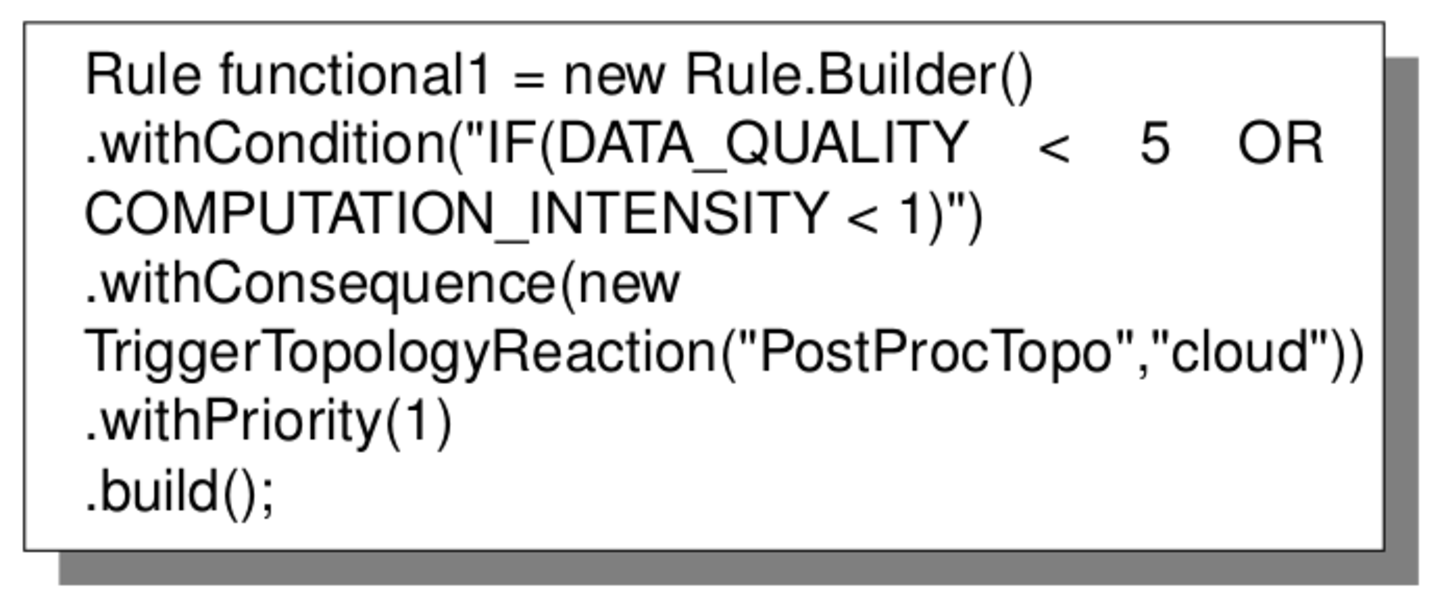
\includegraphics[width=0.7\textwidth]{Figures/RuleTopology.pdf}
  \caption{Trigger topology reaction rule definition.}
  \label{fig:boat1}
\end{figure}


The 'withCondition' is the IF rule expression that has to be satisfied and the 'withConsequence' is the action that will be triggered when the rule is satisfied. The action has two parameters: the first one specifies the name of the topology that needs to triggered if it is the first time executing the action or route to that topology if its already running. The second parameter specifies where it needs to be triggered. In this case it will be triggered on the cloud nodes that are part of the overlay network since its really computationally intensive. 

Another brief code example of how developers will express the content-driven rules to store the matching results at the edge of the network:

\begin{figure}[h!]
  \centering
  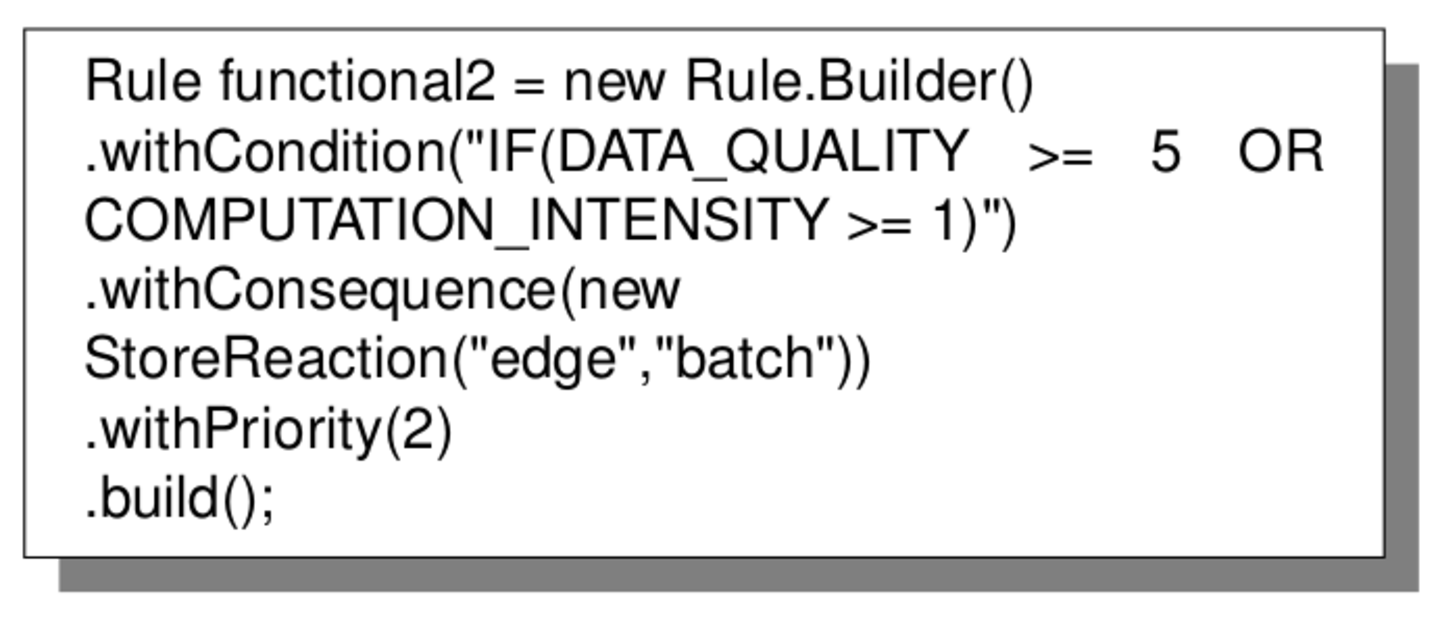
\includegraphics[width=0.7\textwidth]{Figures/StoreReaction.pdf}
  \caption{Store reaction rule definition.}
  \label{fig:boat1}
\end{figure}


The action of this second rule also has two parameters: the first parameter specifies where to store the results of the streaming computation, which in this case, is at one of the edge nodes that are part of the overlay network since we want to be able to get our results quickly. The second parameter specifies how to store the results either one by one (streaming fashion) or batch (several at a time).
\\
\\
Since Apache Storm offers the ability to perform computation in a single tuple at a time and to a group of tuples, we developed two types of Storm data plane bolts: a simple 'IRichBolt' which checks one individual tuple at a time against the rule entries. The second bolt is a 'IWindowedBolt' which checks incoming tuples split into finite sets, or "windows", based on specified criteria such as time and computations, which will be performed on each window of events. Storm developers can now express their data content as an observation overtime (group of tuples). Figure~\ref{fig:win} depicts how to add rules to our rule based windowed bolt.

\begin{figure}[h!]
  \centering
  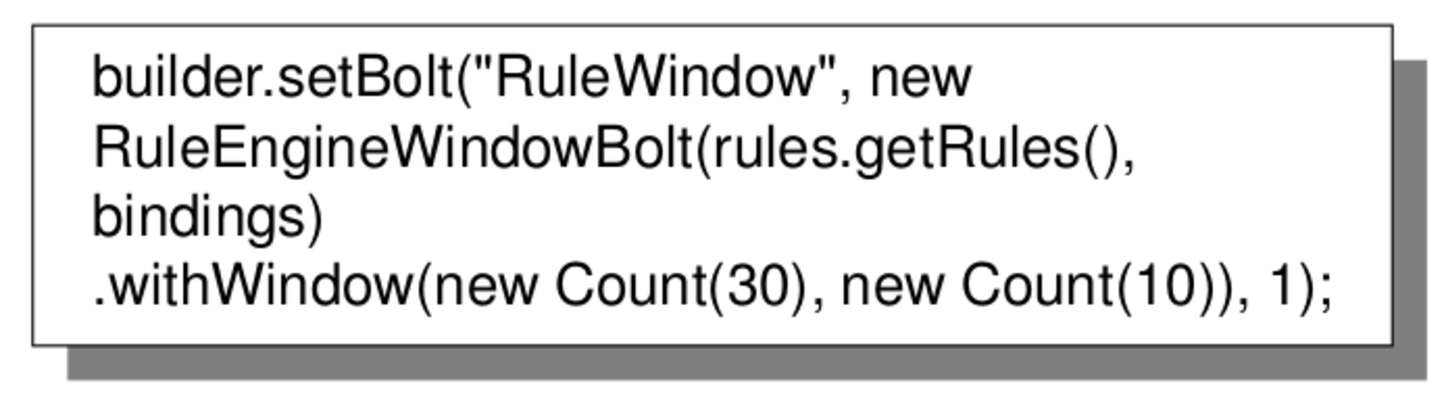
\includegraphics[width=0.7\textwidth]{Figures/WindowBolt.pdf}
  \caption{Rule engine window bolt definition.}
  \label{fig:boat1}
\end{figure}

\subsection{Data Quality Rule-Based System}

\begin{figure}[h!]
  \centering
  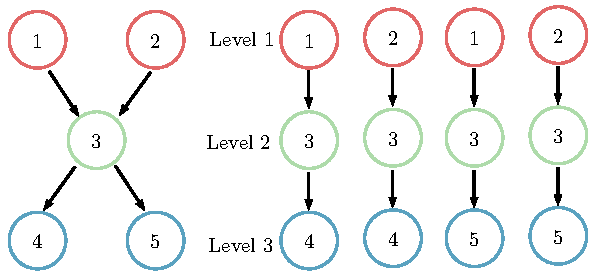
\includegraphics[width=0.6\textwidth]{Figures/AlgoImg.pdf}
  \caption{Storm topology linewise representation}
  \label{fig:boat1}
\end{figure}

From the workflow described in Section \ref{sec:usecase}, if one does not gave time constraints on how fast the data insights are needed, a highest quality of   image will always be the choice. But getting the highest quality results does not guarantee demanding results. For those reasons, we implemented a QoS mechanism to allow Apache Storm developers to specify tradeoffs between quality and computational complexity.

Our data quality rule-based system (QoS rule-based system) works similarly to the content-driven rule-based system. It consists of a custom Apache Storm stream grouping and a rule engine. In Apache Storm, part of defining a topology is to define how data is exchanged between components (how streams are consumed by the bolts). A Stream Grouping specifies which streams are consumed by each bolt. A stream grouping tells a topology how to send tuples between two components. The rule engine parses the given rule entries and computes all the possible paths that will satisfy the constraints specified by the rules. In order for the stream grouping to determine all the paths that will satisfy the constraints specified by the rules we developed in an offline training mode where the stream grouping collects execution information, transfers information, etc.. to determine all the paths that will satisfy the constraint. The data quality rule entries contain a tag filed and a deadline filed. The tag filed needs to be part of each of the tuples that needs to processed. The deadline filed specifies how much time each tuple with the corresponding tag has to go through the entire Storm topology. The algorithm consists of following steps: (1) breakdown the Storm topology into lines-paths from the task of the first level to the task of the last level through only one child on each level; (2) order lines according to their relative computing times $T_{comp}^l$. (3) iterate over the lines until one of the lines does not meet the deadline $D$ and schedule the work.

\begin{figure}[h!]
  \centering
  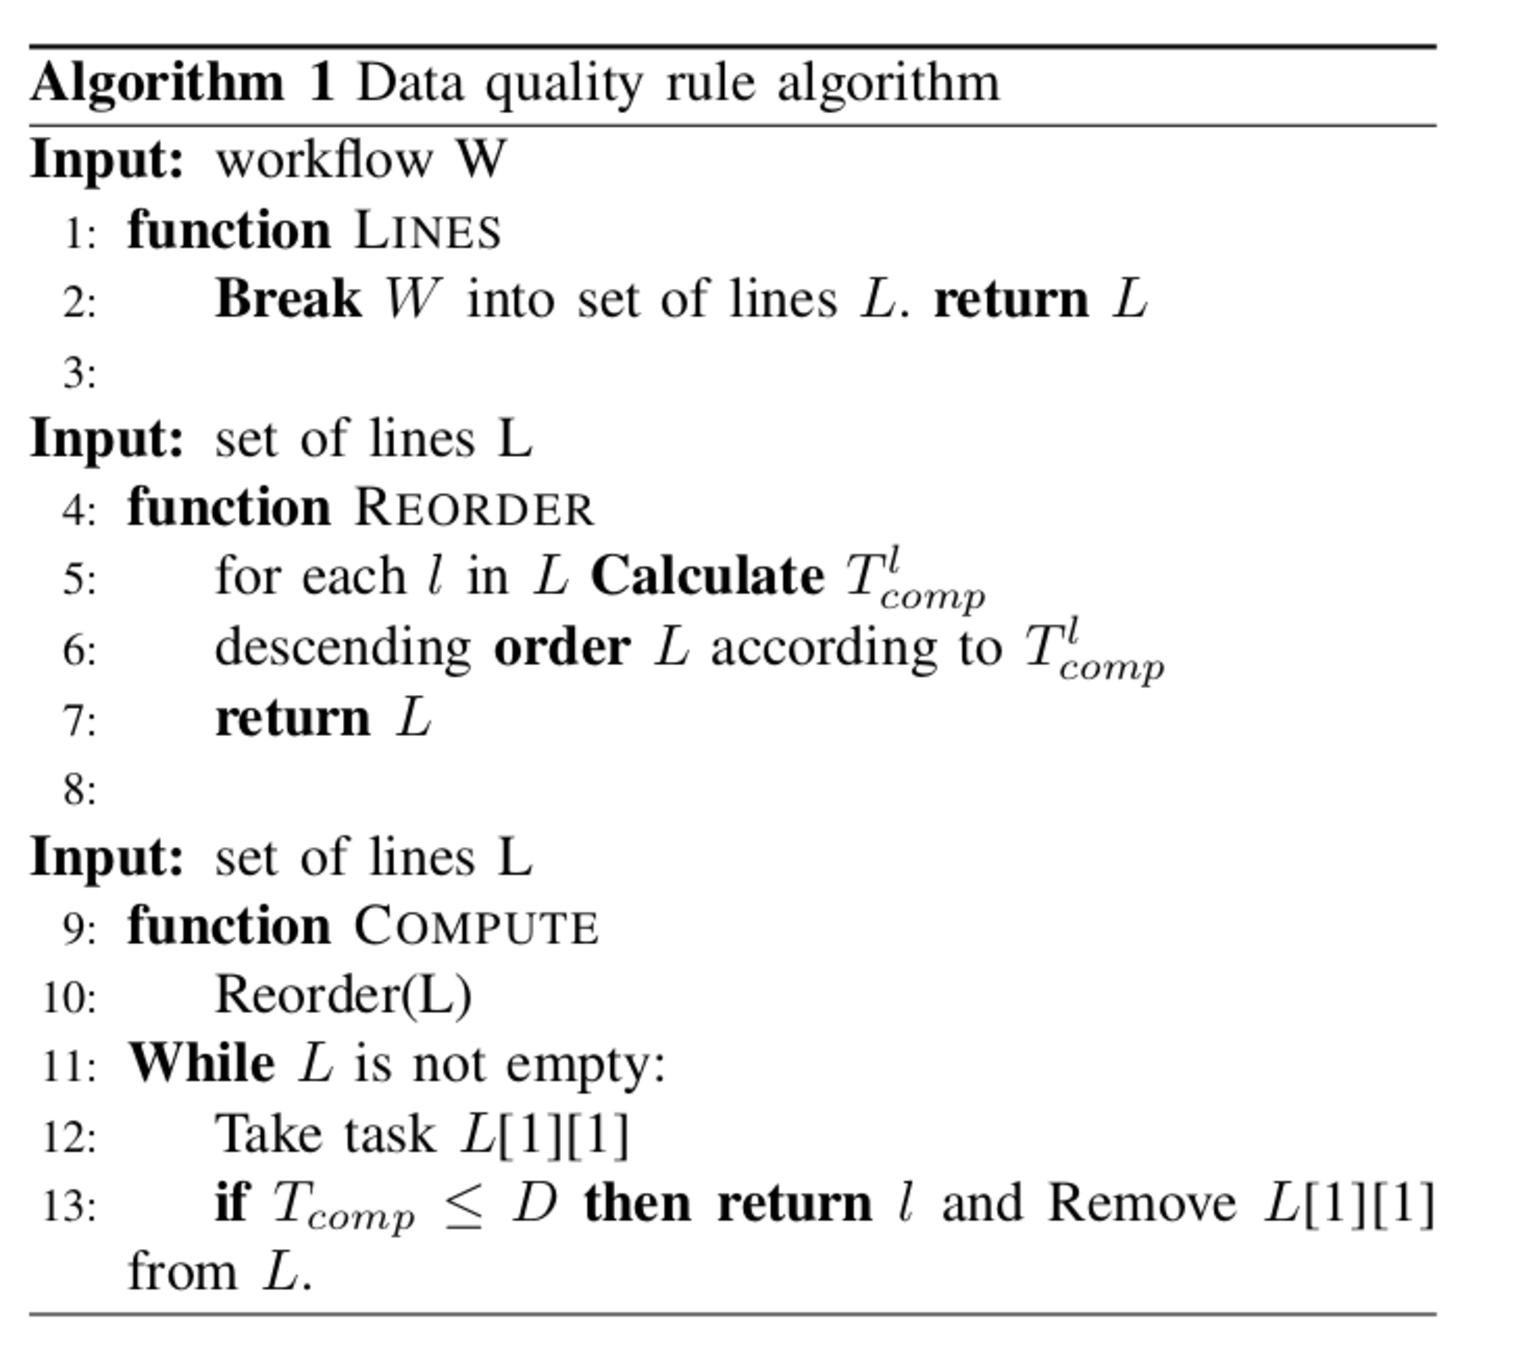
\includegraphics[width=0.7\textwidth]{Figures/Algorithm.pdf}
  \label{fig:boat1}
\end{figure}

The overall steps of the algorithm are depicted in Algorithm 1. In the first step of execution process the algorithm creates lines of the topology tasks and calculates the relative computing time $T_{comp}^l$ for each line. $T_{comp}^l$ is calculated as the sum of execution times $T_{comp}^l$ of all tasks in the line. $T_{comp}^l$ consists of task runtime $T_{run}^t$ and total input data transfer time $T_{data}^t$. Then we order all the paths according to their relative computing times $T_{comp}^l$ so we only need to check if $T_{comp}^l$ satisfies the deadline $D$. Once we find one path that does not satisfy the deadline $D$, we have our set of paths that satisfies the constraint and we schedule the work. The algorithm is constantly running and reschedules the work if the computation conditions change.

Figure~\ref{fig:qosRule} presents a brief code example of how developers will express the data quality rules:

\begin{figure}[h!]
  \centering
  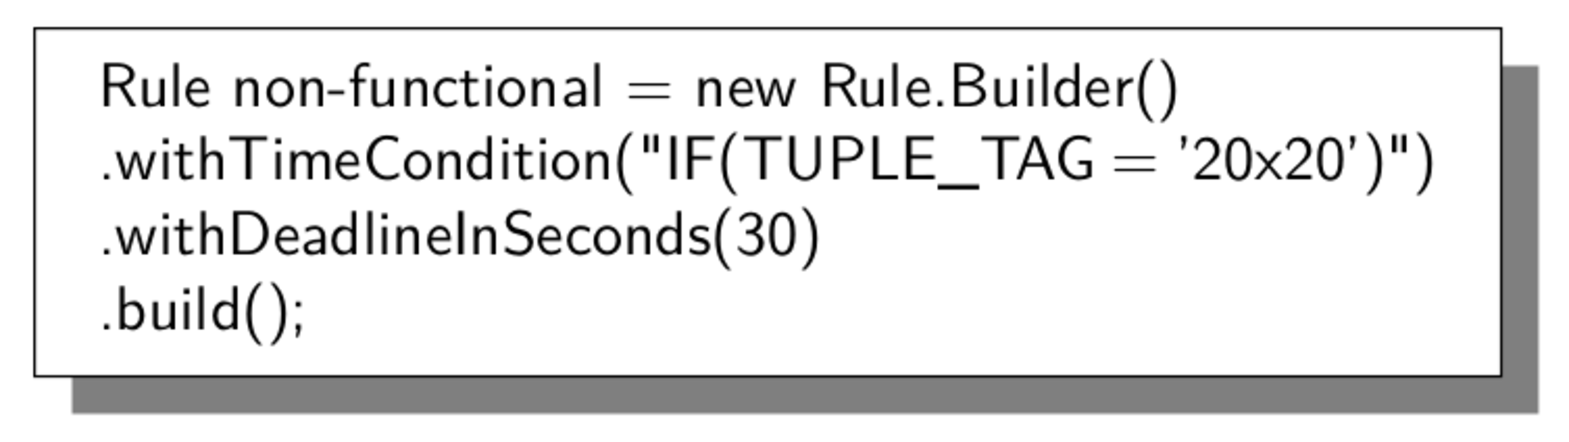
\includegraphics[width=0.7\textwidth]{Figures/qosRule.pdf}
  \label{fig:qosRule}
\end{figure}

%\section{Semantics of the Programming Abstraction}
%\section{Realizing Data-Drive Edge Stream Processing}
%\subsection{Basic Functionality}
%\section{Experimental Evaluation}
%\subsection{Scalability and Overhead Experiments}
%\subsection{Performance experiments}
%\section{Summary}